Chapter \ref{chap:intro} introduced unique characteristics of liquid-fuel
\glspl{MSR}
and highlighted the challenges of modeling liquid-fuel \glspl{MSR} particularly
with older software designed for solid-fuel reactors. In addition, Chapter
\ref{chap:lit} discussed existing \gls{MSR} multiphysics simulation tools and
their capabilities and the noted lack of capabilities for modeling control rod
movement in \glspl{MSR}. Chapter \ref{chap:moltres} illustrated general
features and physics models in Moltres and summarized previous work done with
Moltres for multiphysics modeling of \glspl{MSR}. The latter sections detailed
several limitations in \gls{MSR} multiphysics modeling with
Moltres, including the need for further verification of
Moltres' capabilities, a turbulence model for simulating turbulent flow, and a
control rod modeling capability for transient simulations. In turn,
Chapter \ref{chap:benchmark} detailed a verification study of Moltres for fast-spectrum
\gls{MSR} modeling capabilities by evaluating its performance
through the CNRS benchmark and comparing its results against results from other
\gls{MSR} simulation tools. Lastly, Chapter \ref{chap:hybrid} presented the theory and preliminary
1-D results of the novel Hybrid $S_N$-Diffusion method for improved control rod modeling over
standard neutron diffusion methods.

In this chapter, I will detail the proposed work for the validation of Moltres' \gls{MSR}
modeling capabilities and further enhancements to Moltres to address the
need for a turbulence model and a control rod model in Moltres. The
proposed work contributes towards the overall goal of improving on Moltres' capabilities for
multiphysics modeling of \glspl{MSR} and, by extension, of advanced reactors.
The following sections outline the methods and simulations I will
employ to implement and verify the new capabilities.

\section{Validation of Moltres against the MSRE Pump Start-up and Coast-Down Experiments}

In addition to the completed verification study described in Chapter \ref{chap:benchmark}, I will
perform a \gls{VV} study of Moltres based on the \gls{MSRE} transient flow-rate tests, consisting
of fuel pump start-up and coast-down experiments at zero power criticality. The changing flow rates
cause changes to the \gls{DNP} distribution and the \gls{DNF} in the core. During both
experiments, the reactivity effects of \gls{DNP} drift were measured by
allowing the flux servo controller to maintain criticality. The controller maintains core
criticality by adjusting the control rod position in response to the reactivity effects. The
reactivity effect over time can be calculated by comparing the various control rod positions over
time (Figure \ref{fig:msre-trans}) with the control rod worth curve (Figure \ref{fig:msre-rod})
that was obtained during earlier experiments. I aim to
reproduce the calculated reactivity curve with a Moltres model of the \gls{MSRE}.

\begin{figure}[htb!]
  \centering
  \begin{subfigure}[t]{.49\textwidth}
    \centering
    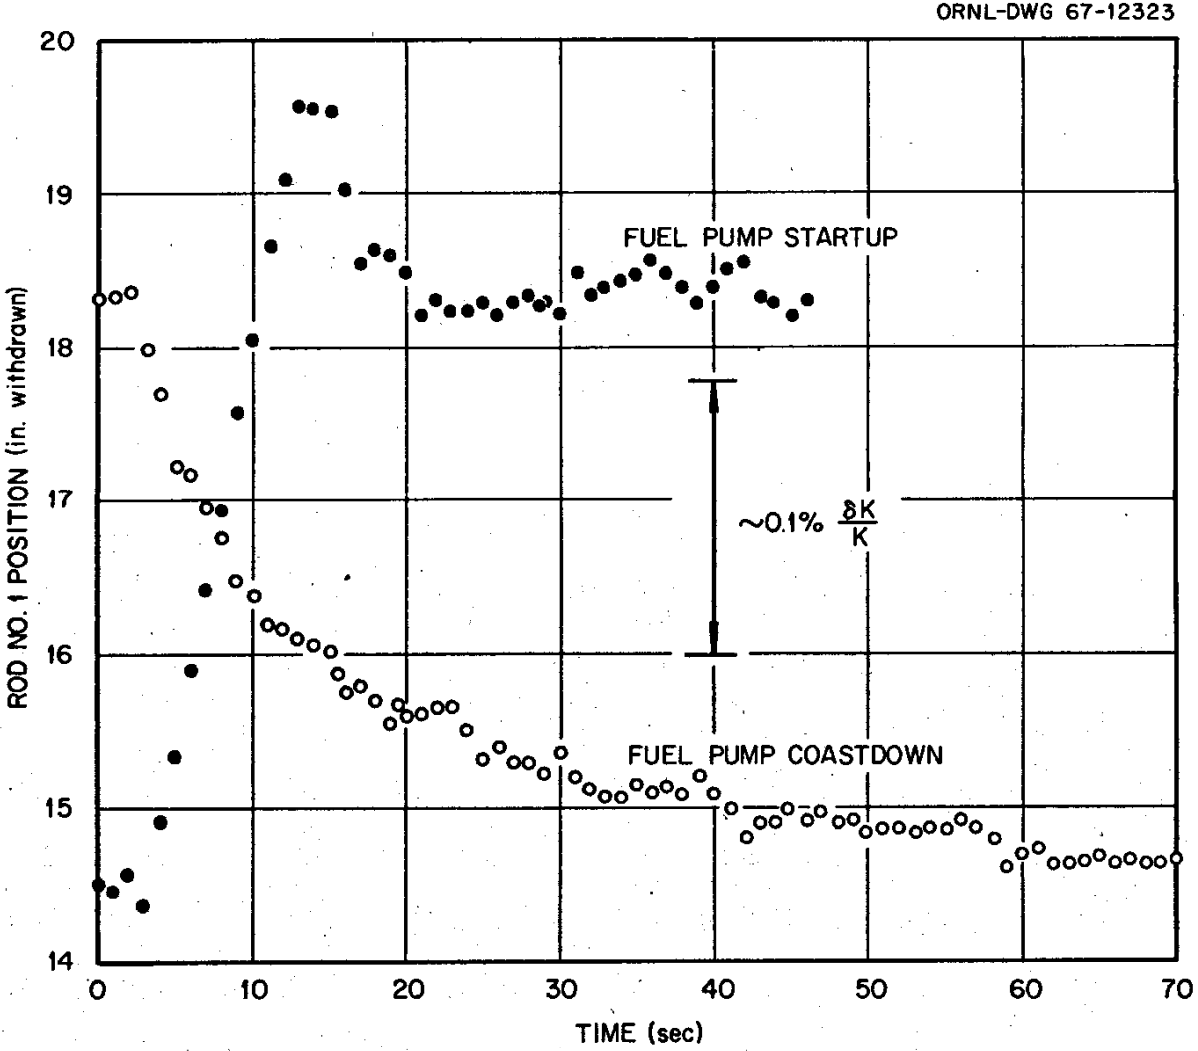
\includegraphics[width=\textwidth]{msre-transient}
    \caption{Control rod response to fuel pump start-up and coast-down.}
    \label{fig:msre-trans}
  \end{subfigure}
  \hfill
  \begin{subfigure}[t]{.49\textwidth}
    \centering
    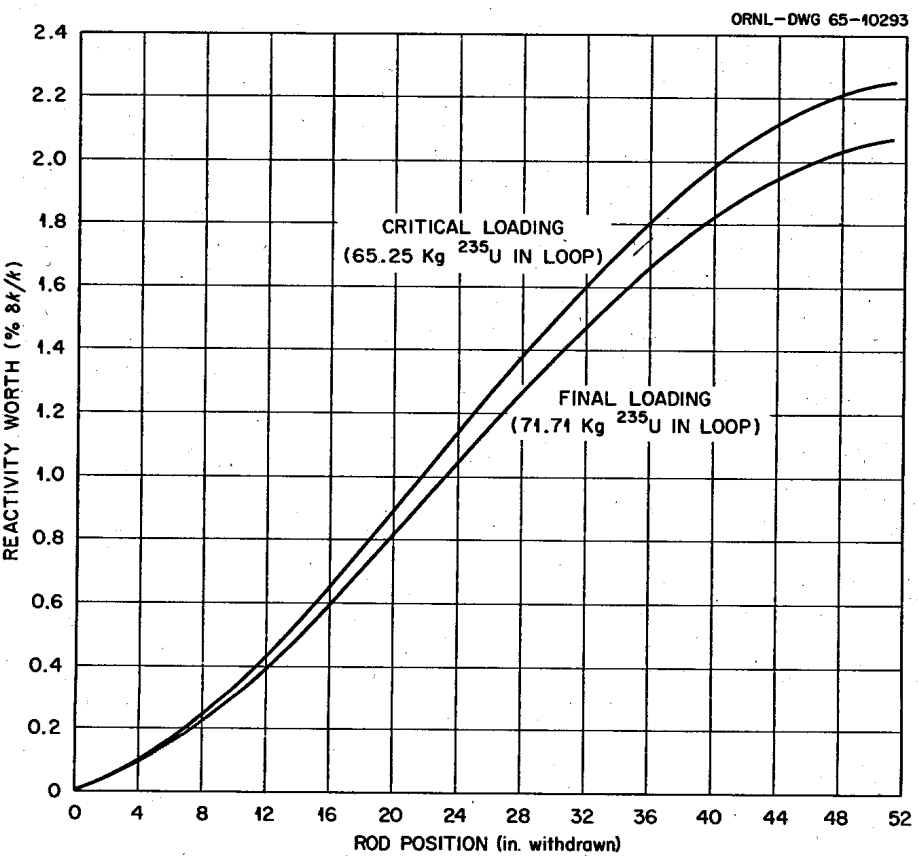
\includegraphics[width=\textwidth]{msre-rod-worth}
    \caption{Integral worth of control rod no. 1.}
    \label{fig:msre-rod}
  \end{subfigure}
\end{figure}

For this study, I will collaborate
with the developer of QuasiMolto \cite{reynolds_analysis_2023}. Therefore, Moltres
will be validated against \gls{MSRE} experimental data and verified against QuasiMolto simulation
results simultaneously. Both QuasiMolto and Moltres models of the \gls{MSRE} will be in R-Z
coordinates as QuasiMolto supports only R-Z \gls{MSR} modeling.

\section{Implementation of a RANS-Based Turbulence Model in Moltres}

I will implement a Spalart-Allmaras turbulence model which falls under the class of
\gls{RANS}-based turbulence models discussed in Chapter \ref{chap:lit}. The
model will be implemented within the \gls{MOOSE} framework and
designed to be compatible with the fluid dynamics modeling infrastructure in
the existing \texttt{Navier-Stokes} module. This approach leverages on the
advanced finite-element solver and multiphysics coupling capabilities in
\gls{MOOSE}.

A comprehensive validation of the implemented model under various types of
turbulent flow falls outside the scope of the proposed work. Instead, I will
focus on verifying and validating its performance under specific flow conditions expected in
liquid-fuel \glspl{MSR}---wall-bounded turbulent flow with flow separation past
sharp changes in the flow channel geometry. The backward facing step is a
widely known fluid dynamics problem commonly used to assess the accuracy of
turbulence model solvers \cite{lasher_computation_1992}.
The problem domain features a straight duct
on the left followed by a sudden back step in the lower wall which causes flow
separation. The flow eventually reattaches and recovers downstream of the step.
I will simulate and validate against experimental data from Driver \&
Seegmiller \cite{driver_features_1985}. Quantities of interest from this
exercise are the spatial distributions of the velocity components, turbulent
kinetic energy, and eddy viscosity, and the reattachment length of the
turbulent shear layer.

\section{Development of a Novel Hybrid Method to Improve Control Rod Modeling in Moltres}

In Chapter \ref{chap:hybrid}, I presented the theory and preliminary results of the Hybrid
$S_N$-Diffusion method for several 1-D \gls{MSRE}-like, graphite-moderated geometries. The hybrid
method generates \glspl{SVDC}, which provide pointwise corrections to the diffusion subsolver, from
the $S_N$ subsolver neutron current and flux gradient solutions. The hybrid method minimizes
computational costs by imposing the $S_N$ calculations on a small subdomain centered on the control
rod region and relaxing the $S_N$ subsolver convergence tolerance since the neutron current and
flux gradient converges faster than the neutron flux. As intended,
the hybrid method provided better multiplication factor and neutron flux estimates over the
standard neutron diffusion method in systems containing control rods.

The preliminary investigations also brought up several concerns to be addressed in addition to
broader subobjectives, all of which are listed below in approximate chronological order:
%
\begin{itemize}
  \item Develop a robust submethod for resolving \glspl{SVDC} near neutron flux peaks and troughs,
    or an alternative streaming correction term formulation to avoid \gls{SVDC} singularities.
  \item Implement the hybrid method in Moltres.
  \item Extend the hybrid method for 2-D and 3-D reactor modeling.
  \item Investigate and rectify potential rod cusping errors, which arise from non-alignment of
    the control rod boundary with mesh element boundaries when modeling time-dependent control rod
    insertion/withdrawal.
  \item Perform a \gls{VV} study of the hybrid method by demonstrating it on a Moltres
    \gls{MSRE} model, and comparing it against a reference OpenMC \gls{MSRE} model and \gls{MSRE}
    experimental data.
  \item Characterize and compare the computational efficiencies of the hybrid method implemented as
    multilevel and multischeme methods. If the multi-scheme implementation is viable, it could
    reduce computational costs by running the $S_N$ and diffusion subsolvers concurrently and
    eliminating outer iterations.
\end{itemize}

In this context, multilevel neutronics methods refer to methods that apply different neutronics
methods on the same or overlapping problem domains with data exchanges between the subsolvers to
improve accuracy or convergence rates. On the other hand, multischeme neutronics methods refer to
methods that apply different neutronics methods on non-overlapping subdomains to take advantage of
higher fidelity or convergence rates associated with the methods under different conditions. While
I initially formulated the Hybrid $S_N$-Diffusion method as a multilevel (two-level) method, it
could be adapted to be a multischeme method with some overlap to improve flux estimates near the
subdomain interfaces.
